\documentclass[mathserif]{beamer}
\usepackage{beamerthemeshadow}
\usepackage{beamerthemesplit}
%\usetheme{shadow}
\usecolortheme{default}
\setbeamertemplate{footline}[frame number]
\useinnertheme[shadow=true]{rounded}
%\setbeamertemplate{footline}{\insertframenumber/\inserttotalframenumber}
%\useoutertheme{infolines}
%\setbeamertemplate{headline}{} % removes the headline that infolines inserts

%\usetheme{boxes}
%\usepackage{amsmass}
%\usepackage{amssymb,amsfonts,url}


\usepackage{algorithm}
\usepackage{algorithmic}

\usepackage{graphicx}
\graphicspath{{Problems/}}
%\usepackage{CJK}
%\usepackage{pinyin}

%    \begin{figure}
%        \centering
%        \includegraphics[width=0.8\textwidth]{newGeneRep.eps}
%    \end{figure}

% \begin{figure}%
%   \begin{center}%
%     \begin{minipage}{0.70\textwidth}%
%      \includegraphics[width=1.0\textwidth]{comp25000.eps}%
%     \end{minipage}%
%     \begin{minipage}{0.30\textwidth}
%      \includegraphics[width=1.0\textwidth]{comparelabel.eps}%
%     \end{minipage}%
%   \end{center}
% \end{figure}

% \begin{table}
%   {\begin{tabular}{l|rrr}\hline
%       & \multicolumn{3}{c}{Actual number of DCJ operations}\\
%       \# genes &\# genes $\times 1$&\# genes $\times 2$&\# genes  $\times 3$ \\
% \hline
%      (a)~25,000 & 0.5\% ~~&  0.9\% ~~& 1.7\%~~\\
%       (b)~10,000 & 0.8\%~~ &  1.4\% ~~& 2.7\%~~\\
%      (c)~ 1,000 & 2.7\%~~ & 4.7\%~~ & 14.7\%~~\\ \hline
%     \end{tabular}} {}%
% \end{table}

% \begin{eqnarray}
% T(n) &=&  \sum\nolimits_{i=1}^n C_i \\
%      &=&  \# PUSH + \#POP \\
%      &<& 2\times \#PUSH \\
%      &<& 2n \\
% \end{eqnarray}

% \[ 
% \begin{matrix}
% \begin{pmatrix}
% C_{11} & C_{12} \\ 
% C_{21} & C_{22} 
% \end{pmatrix}
% =
% \begin{pmatrix}
% A_{11} & A_{12} \\ 
% A_{21} & A_{22}  
% \end{pmatrix}
% 
% \begin{pmatrix}
% B_{11} & B_{12} \\ 
% B_{21} & B_{22}  
%  
% \end{pmatrix}
%     
%    \end{matrix}
% \]
% 
% 
% \begin{eqnarray}
%  C_{11} &=& (A_{11}\times B_{11}) + (A_{12} \times B_{21}) \\
% C_{12} &=& (A_{11}\times B_{12}) + (A_{12} \times B_{22}) \\
% C_{21} &=& (A_{21}\times B_{11}) + (A_{22} \times B_{21}) \\
% C_{22} &=& (A_{21}\times B_{12}) + (A_{22} \times B_{22}) 
% \end{eqnarray}
% \begin{figure}%
%      \begin{minipage}{0.32\textwidth}%
%       \includegraphics[width=1.0\textwidth]{L7-intervalschedulingdpalgorithm.eps}%
%      \end{minipage}%
%  \quad
%      \begin{minipage}{0.30\textwidth}
%       \includegraphics[width=1.0\textwidth]{L7-intervalschedulinggreedyalgorithm.eps}%
%      \end{minipage}%
%  \quad
%       \begin{minipage}{0.25\textwidth}
%       \includegraphics[width=1.0\textwidth]{L7-intervalschedulinggreedyalgorithm2.eps}%
%      \end{minipage}%
% 
%  \end{figure}

\title{CS612  Algorithm Design and Analysis }
\subtitle{ Lecture 15. {\sc Selection} problem 
\footnote{The slides are made based on Randomized Algorithm by R. Motwani and P. Raghavan, and a lecture by T. Chan. } }
\author{Dongbo Bu \\
\ \\
{\small Institute of Computing Technology \\ 
Chinese Academy of Sciences, Beijing, China}}

\date{}

\begin{document}
%\begin{CJK}{UTF8}{cyberbit}

\frame[allowframebreaks]{\titlepage}

\frame{
\frametitle{Outline}
\begin{itemize}
\item Introduction
\item Several lower bounds;
\item Algorithms for selection:
\begin{enumerate}
\item Deterministic $O(n)$ algorithm;
\item A randomized divide-and-conquer $O(n)$ algorithm;
\item A random sampling algorithm.
\end{enumerate}
\end{itemize}

\begin{footnotesize}
Note: 
\begin{itemize}
 \item \textcolor{red}{The natural brute-force algorithm is already polynomial time; divide-and-conquer is serving to reduce the running time to a lower polynomial. }
 \item \textcolor{red}{Divide-and-conquer becomes more powerful when combined with randomization. }
 \item \textcolor{red}{Given a large dataset, it might be useful to randomly sample a small set first. We can perform computation on this small set using brute-force algorithm, and finally generralize observations to the whole dataset.}
\end{itemize}
\end{footnotesize}
}

\frame{
\begin{block}{}
 Introduction
\end{block}
}


\frame{
\frametitle{ {\sc Selection } problem }
\begin{block}{}
{\bf INPUT: } \\
Given a set of number $S=\{a_1,a_2,...,a_n\}$, and a number $k\leq n$;  \\
{\bf OUTPUT: } \\ 
the $k$-th smallest item in general case (or the median of $S$ as a specical case).
\end{block}

For example, given a set $S=\{18, 15, 27, 13, 1, 7, 25\}$, the objective is the median of $S$. 

Note: 
\begin{itemize}
 \item A feasible strategy is to sort $S$ first, and then report the $k$-th one, which takes $O(n\log n)$ time. 
 \item It is possible to develop a faster algorithm by using divide-and-conquer technique, say the deterministic linear algorithm ($16n$ comparisons) by Blum et al.  
\end{itemize}
}

\frame{
\begin{block}{}
 Deterministic algorithm
\end{block}
}

\frame{
\frametitle{ A general divide-and-conquer paradigm }
Algorithm $Select( S, k )$: 
\begin{algorithmic}[1]
\STATE Choose an item $s_i$ from $S$ as a pivot; 
\STATE $S^+ = \{\}$; 
\STATE $S^- = \{\}$; 
\FOR { $j=1$ to $n$ }
\IF { $s_j > s_i $ }
\STATE $S^+ = S^+ \cup \{s_j\}$; 
\ELSE
\STATE $S^- = S^- \cup \{s_j\}$; 
\ENDIF
\ENDFOR
\IF{ $|S^-| = k-1 $} 
\RETURN $s_i$;
\ELSIF { $|S^-| = k-1 $} 
\RETURN $Select( S^-, k )$;
\ELSE 
\RETURN $Select( S^+, k - | S^- | +1  )$;
\ENDIF
\end{algorithmic}
}

\frame{
\frametitle{ Perform iteration on ONLY one subset. }

%  \begin{figure}
%         \includegraphics[width=3in]{L12-randomizedkmedianalgorithm.eps}
%  \end{figure}

Intuition: 
\begin{enumerate}
 \item 
At first, an element $a_i$ is chosen to split $S$ into two parts $S^+=\{a_j: a_j \geq a_i\}$, and $S^-=\{a_j: a_j < a_i\}$. 
\item 
We can determine whether the $k$-th median is in $S^+$ or $S^-$. 
\item 
Thus, we perform iteration on ONLY one subset.
\end{enumerate}
} 


\frame{
\frametitle{ How to choose a splitter? }
We have the follow options: 

\begin{itemize}
\begin{small}
 \item Bad choice: select the smallest element at each iteration. 
$T(n)=T(n-1)+O(n) = O(n^2)$
 \item Ideal choice: select the median at each iteration. 
$T(n)=T(\tfrac{n}{2})+O(n)=O(n)$
 \item Good choice: select a ``centered'' element $a_i$, i.e., $|S^+| \geq \epsilon n$, and $|S^-| \geq \epsilon n$ for a fixed $\epsilon > 0$. 
\end{small}
\begin{small}
\begin{eqnarray}
T(n) &\leq& T( (1-\epsilon)n) + O(n) \nonumber \\
     &\leq& cn+c(1-\epsilon)n+c(1-\epsilon)^2n+.... \nonumber \\
     &=& O(n) \nonumber \\
\end{eqnarray}
\end{small}
\end{itemize}
e.g.: $\epsilon=\frac{1}{4}$: 
\begin{figure}
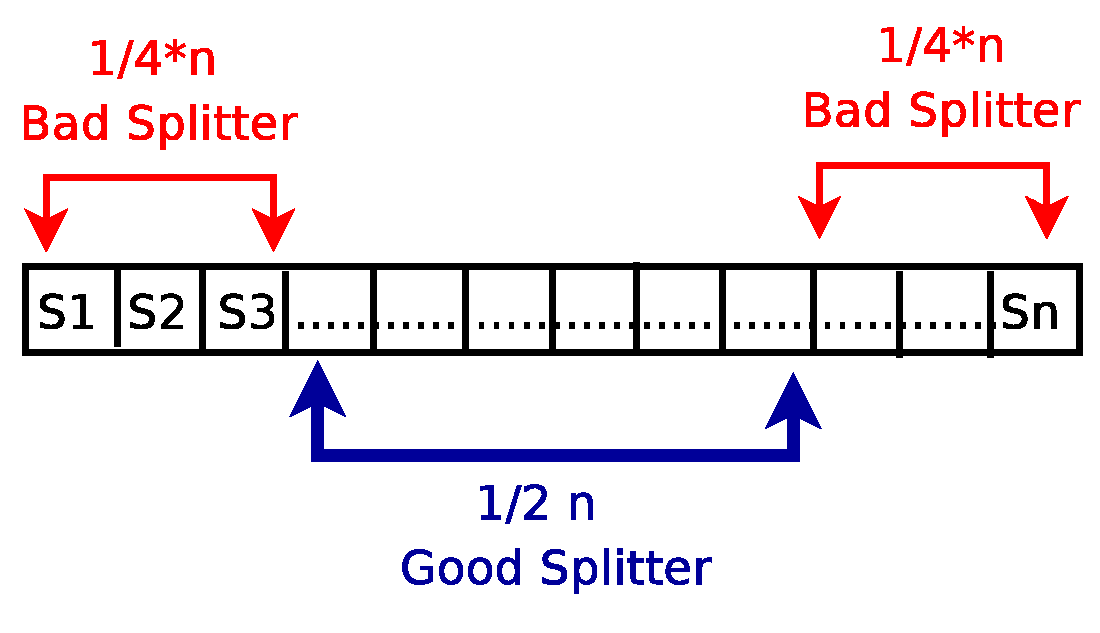
\includegraphics[width=1.8in]{L12-randomdcsplitter.eps}
\end{figure}
} 



\frame[allowframebreaks]{
\frametitle{ BFPRT algorithm: a linear deterministic algorithm } 
\begin{itemize}
  \item Still using the idea of choosing splitter. The ideal splitter is the median; however, finding the median is exactly our objective. 
 \item Thus, just try to get ``something close to the median'', say within $\tfrac{n}{4}$ from the median. 
 \item How can we get something close to the median? Instead of finding the median of the \textcolor{red}{``whole set''}, find a median of a \textcolor{red}{``sample''}. 
 \item But how to choose a sample? Medians again!
\end{itemize}

} 

\frame{
\frametitle{ Median of medians algorithm [Blum, 1973] }

``Median of medians'' algorithm: \\
\begin{algorithmic}[1]
\STATE  Line up elements in groups of 5 elements; 
\STATE  Find the median of each group; (takes $O(\tfrac{6n}{5})$ time)
 \STATE Find the median of medians (denoted as $M$); (takes $T(\frac{n}{5})$ time)
 \STATE Use $M$ as splitter to partition the input and call the algorithm recursively on one of the partitions. 
\end{algorithmic}

 \begin{figure}
        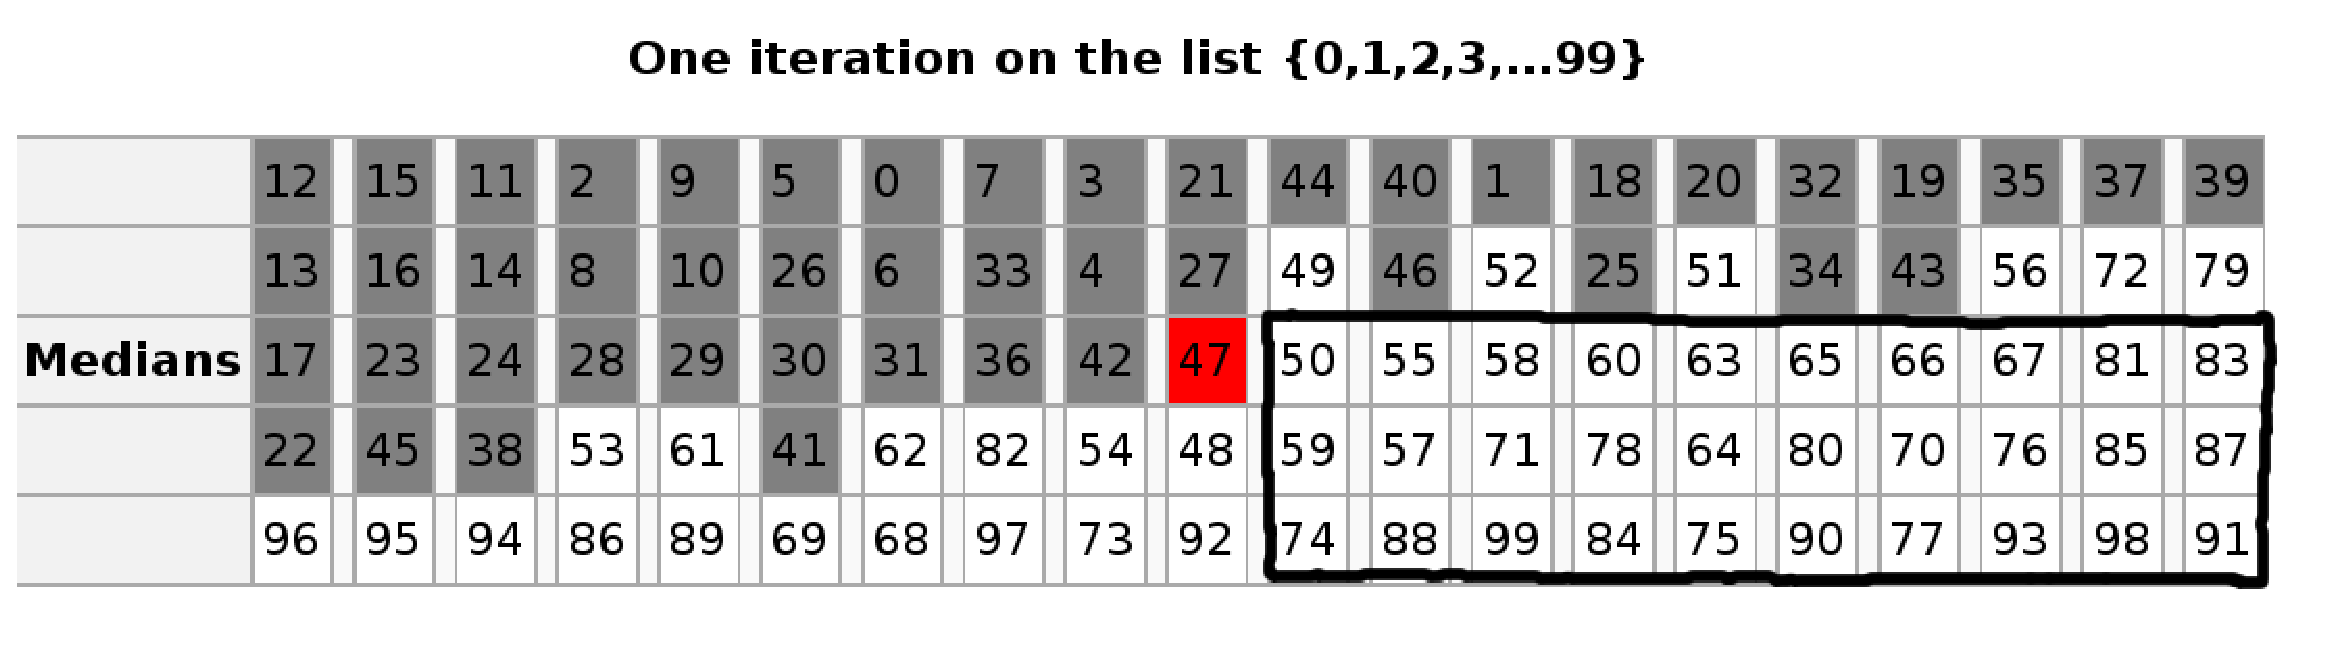
\includegraphics[width=3.5in]{L15-selection.eps}
 \end{figure}

Analysis:

$T(n)=T(\tfrac{n}{5}) + T(\tfrac{7n}{10}) + \tfrac{6n}{5}$ at most $24n$ comparisons. 

(here, $\tfrac{7n}{10}$ comes from the fact that at least $\tfrac{3n}{10}$ can be deleted by using $M$ as the splitter. )
}


\frame{
\begin{block}{}
 Divide-and-conquorer with random pivoting 
\end{block}
}

\frame{
\frametitle{ Randomized divide-and-conquorer}

Algorithm $RandomSelect(n, k)$: 
\begin{algorithmic}[1]
\STATE Choose an element $s_i$ from $S$ uniformly at random; 
\STATE $S^+=\{\};$;
\STATE $S^-=\{\};$;
\FOR { $j=1$ to $n$ }
\IF { $s_j > s_i $ }
\STATE $S^+ = S^+ \cup \{s_j\}$; 
\ELSE
\STATE $S^- = S^- \cup \{s_j\}$; 
\ENDIF
\ENDFOR
\IF{ $|S^-| = k-1 $} 
\RETURN $s_i$;
\ELSIF { $|S^-| = k-1 $} 
\RETURN $RandomSelect( S^-, k )$;
\ELSE 
\RETURN $RandomSelect( S^+, k - | S^- | +1  )$;
\ENDIF
\end{algorithmic}
}

\frame{
\frametitle{ Randomized divide-and-conquorer cont'd}

e.g.: $\epsilon=\frac{1}{4}$: 
\begin{figure}
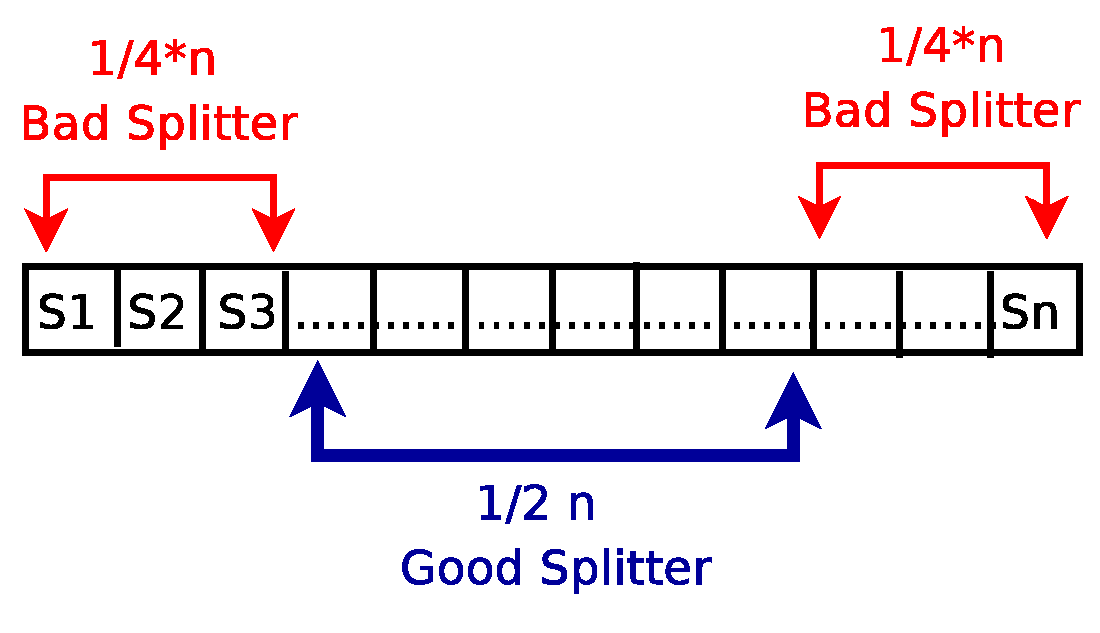
\includegraphics[width=2.5in]{L12-randomdcsplitter.eps}
\end{figure}

Key observation: if we choose a splitter $a_i \in S$ uniformly at random, it is easy to get a good splitter since a fairly large fraction of the elements are ``centered''. 
} 

\frame{
\frametitle{ Randomized divide-and-conquorer cont'd}

\begin{small}
\begin{Theorem}
 The expected running time of Select(n,k) is $O(n)$.
\end{Theorem}
\begin{Proof}
 \begin{itemize}
  \item Let $\epsilon=\tfrac{1}{4}$. We'll say that the algorithm is in phase $j$ when the size of set under consideration is in $[n(\tfrac{3}{4})^{j-1}, n(\tfrac{3}{4})^{j}]$. 
  \item Let $X$ be the number of steps. And $X_j$ be the number of steps in phase $j$. Thus, $X=X_0+X_1+...$. 
  \item Consider the $j$-th phase. The probability to find a centered splitter is $\geq \tfrac{1}{2}$ since  at least half elements are centered. Thus, the expected number of iterations  to find a centered splitter is: $2$. 
  \item Each iteration costs $cn(\tfrac{3}{4})^j$ steps since there are at most $n(\tfrac{3}{4})^j$ elements in phase $j$. Thus,  $E(X_j)\leq 2 cn(\tfrac{3}{4})^j$.
  \item $E(X) = E(X_0 + X_1 + ....) \leq \sum_j 2cn (\tfrac{3}{4})^j \leq 8cn$.  
 \end{itemize}
\end{Proof}
\end{small}
}

\frame{
\begin{block}{}
 Random sampling strategy for selection
\end{block}
}

\frame{
\frametitle{ A ``random sampling'' algorithm [Floyd \& Rivest, 1975]}

Basic idea: randomly sample a subset as a representation of the whole set. \\

Random sampling algorithm:  
\begin{algorithmic}[1]
\STATE  randomly sample $r$ elements (with replacement) from $S=\{s_1,s_2,...,s_n\}$. Denote the $r$ elements as $R$.
\STATE  take the $(1-\delta)\frac{r}{2}$-th smallest element of $R$ (denoted as $a$), and the $(1+\delta)\frac{r}{2}$-th smallest element of $R$ (denoted as $b$); 
 \STATE  divide $S$ into three dis-joint subsets:
\begin{eqnarray*}
L &=& \{s_i : s_i < a \}; \\
M &=& \{s_i : a \leq s_i \leq b \}; \\
H &=& \{s_i : s_i > b \}; 
\end{eqnarray*}
  \STATE  check $|L| \leq \frac{n}{2}$, $|H| \leq \frac{n}{2}$, and $|M| \leq c \delta n$. If not, goto Step 1. 
 \STATE  return the $(\frac{n}{2} - |L|)$-th smallest of $M$; 
\end{algorithmic}
}

\frame{
\frametitle{ Example }
\begin{figure}
        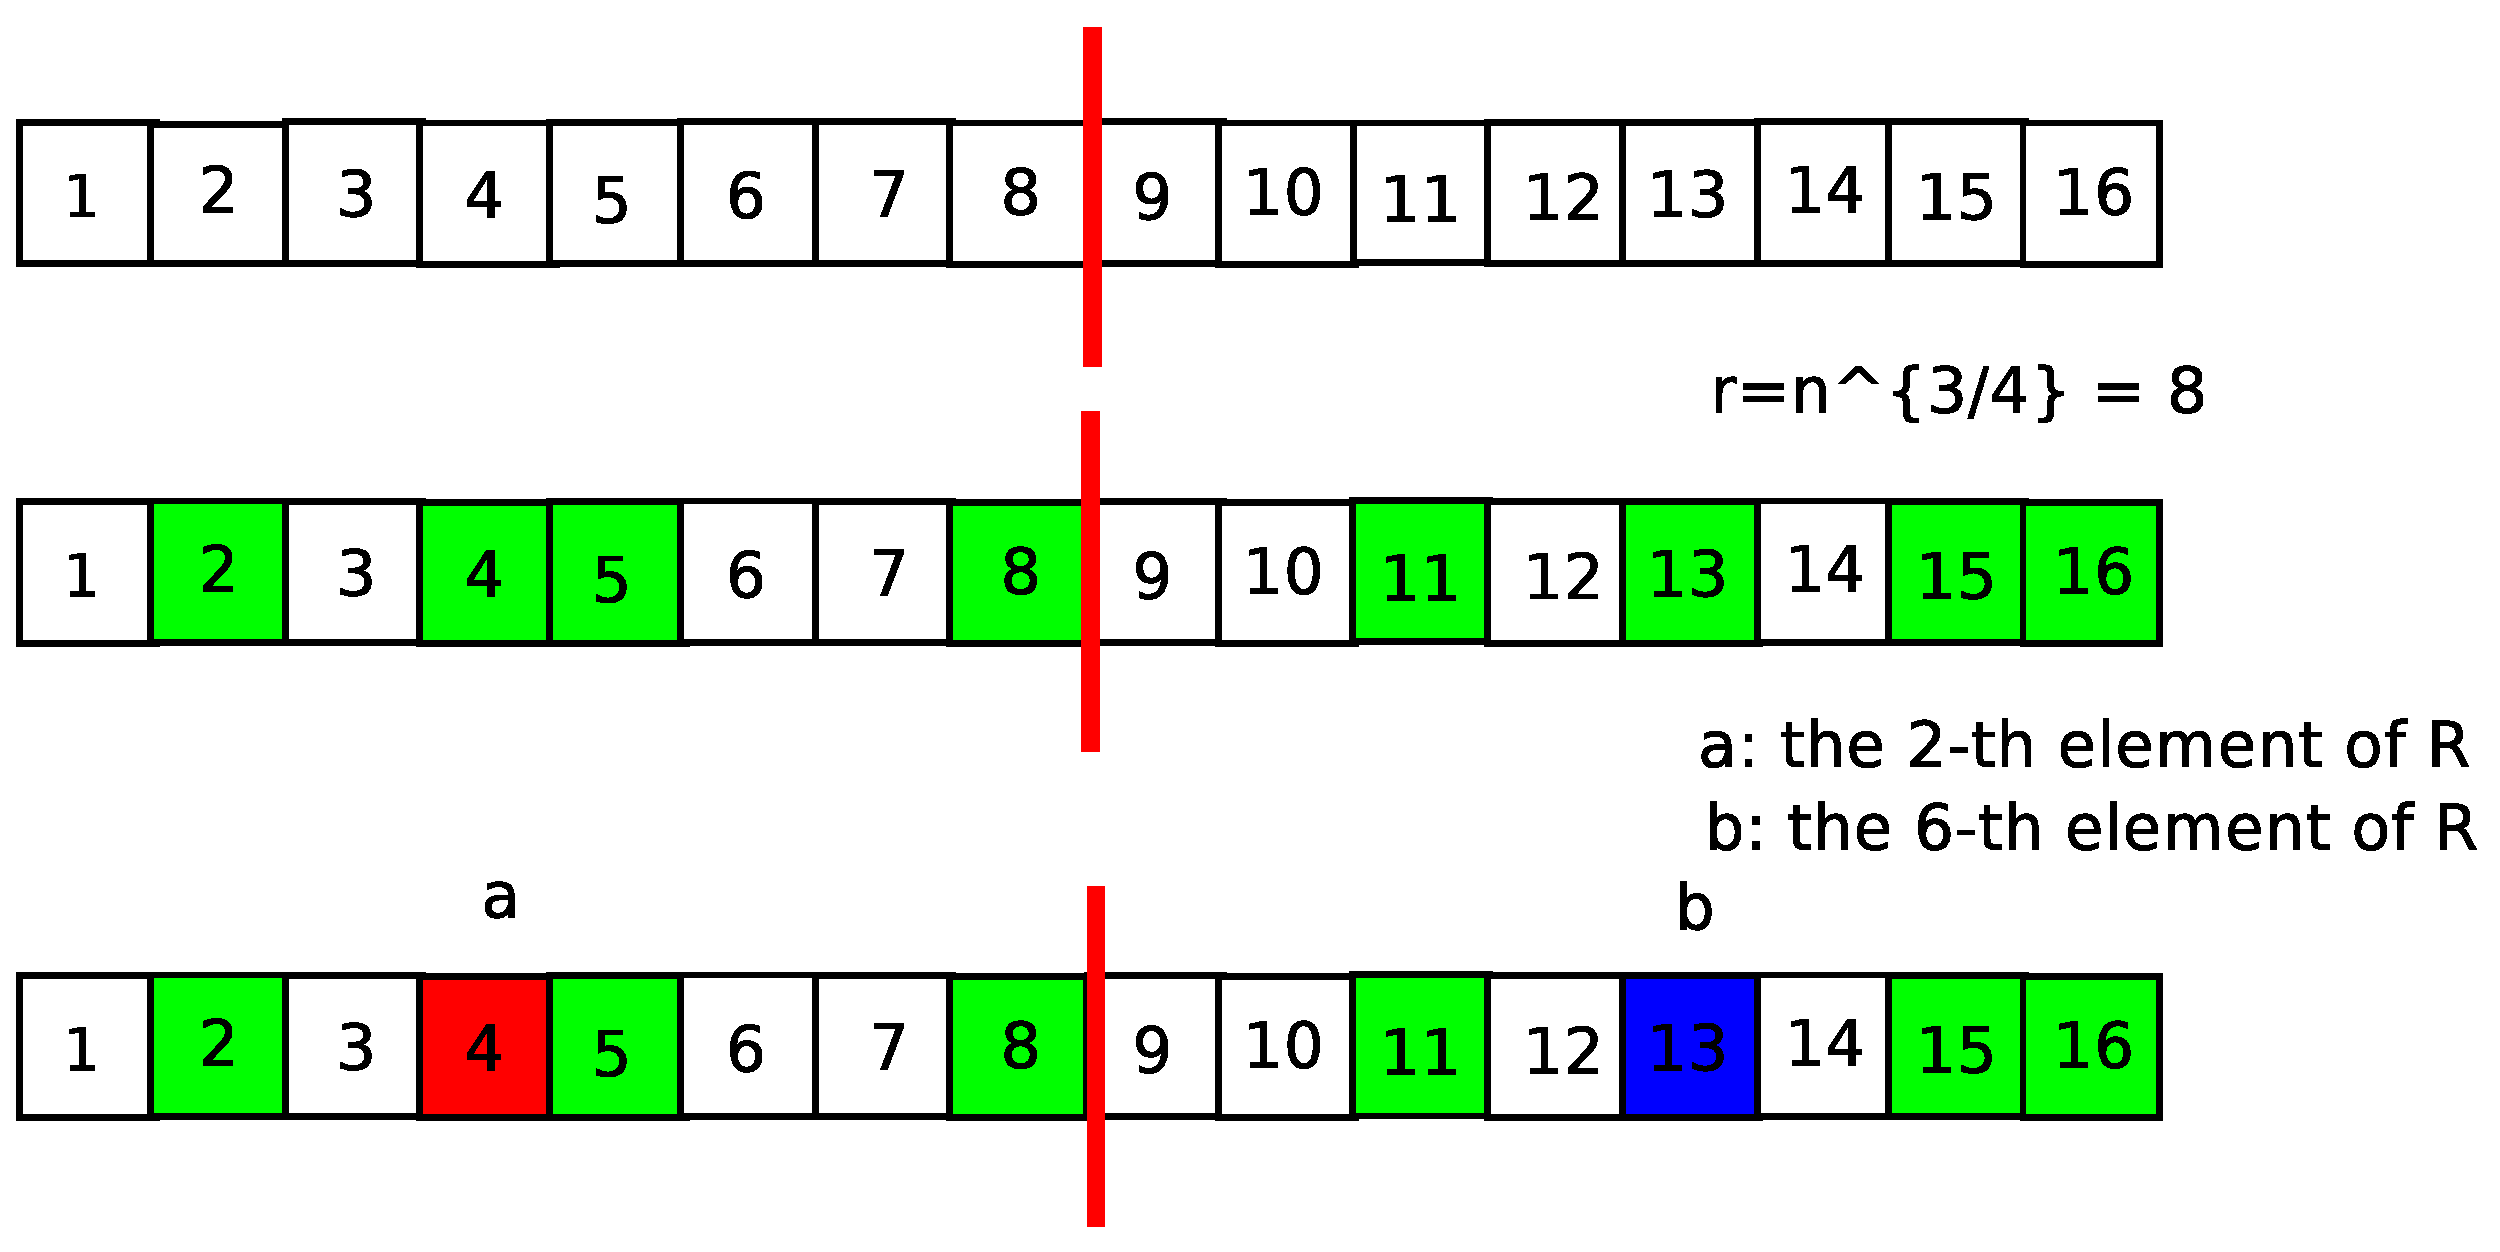
\includegraphics[width=3.5in]{L15-randomsampling.eps}
\end{figure}

Two requirements of $M$: 
\begin{itemize}
\item On one side, $M$ should be LARGE enough such that the median is covered by $M$ with a high probability; 
\item On the other side, $M$ should be SMALL enough such that Step 4 will not take a long time; 
\end{itemize}
}

\frame{
\frametitle{ Time-comlexity analysis } 
Running time: 
\begin{itemize}
 \item Step 2: $O( r \log r ) = o(n)$; (sorting $R$)
 \item Step 3: $ 2n $ steps. ($O(n) + O(|M| + |H|)$)
 \item Step 4: $O( \delta n \log (\delta n) )$. 
\end{itemize}
Setting $r=n^{\frac{3}{4}}$, and $\delta = n^{-\frac{1}{4}}$. The time bound of Step 4 changes to: \\

\begin{itemize}
 \item Step 4: $O( \delta n \log (\delta n) ) = o( n )$. 
\end{itemize}

Total steps: $2n + o(n)$. \\
\begin{itemize}
 \item 
The best known deterministic algorithm: $3n$. But too complicated. 
 \item 
A lower bound: $2n$. 
\end{itemize}
}

\frame[allowframebreaks]{
\frametitle{ Error probability analysis }
\begin{Theorem}
With probability $1-O(n^{-\frac{1}{4}})$, the $RandomSamplingSelect$ algorithm reports the median in the first pass. Thus, the running time is only $2n+o(n)$.  
\end{Theorem}

\begin{figure}
        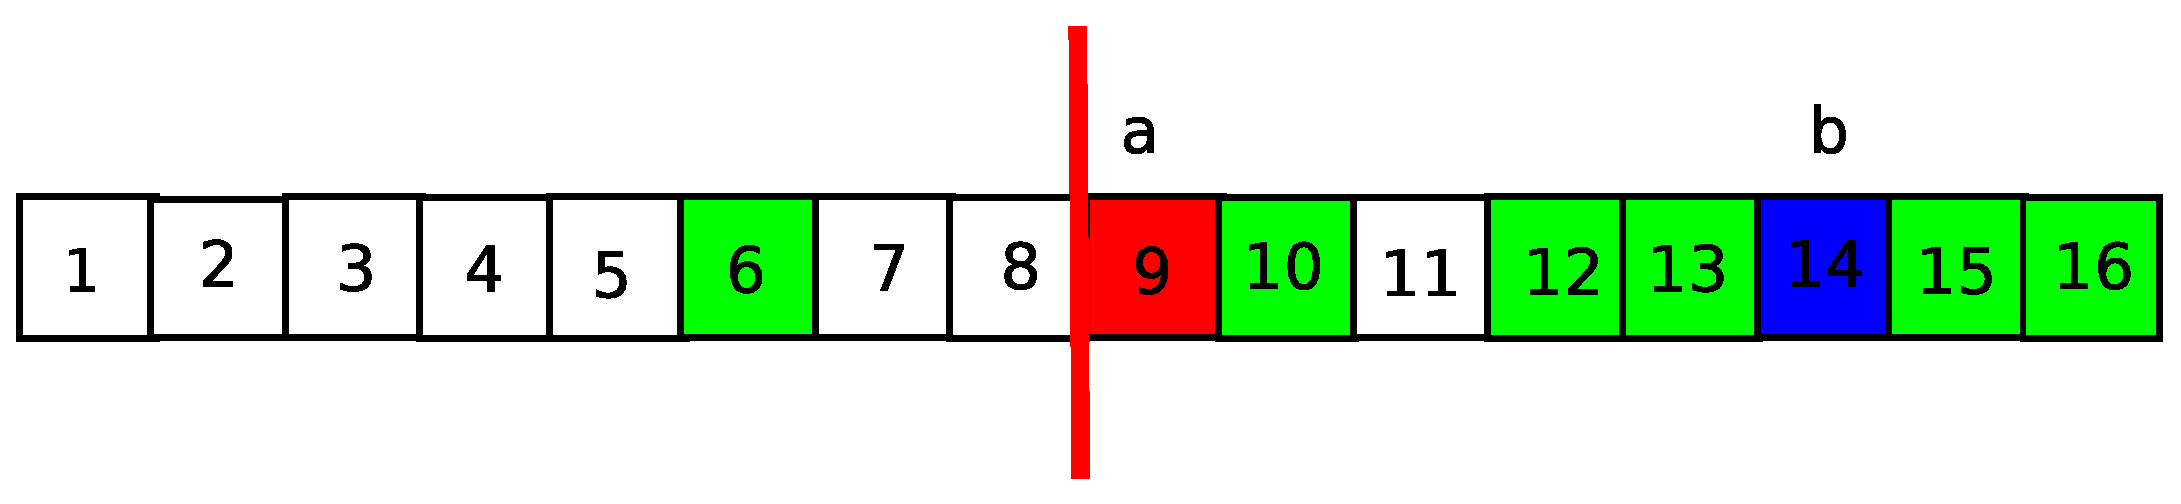
\includegraphics[width=3.5in]{L15-randomsamplingcase1.eps}
 \end{figure}

Three cases of failure in Step 4: \\
Case 1: \\
Define index variable $x_i=1$ when the $i$-th sample is less than the median, and $x_i=0$ otherwise. Let $X=x_1+...+x_r$ be the number of samples that is less than the median. We have: 
$E(x_i) = \tfrac{1}{2}$ and $\sigma^2(x_i) = \tfrac{1}{4}$. \\
$E(X) = \tfrac{1}{2}r$ and $\sigma^2(X) = \tfrac{1}{4} r$. 
\begin{eqnarray} 
\Pr( |L| \geq \tfrac{n}{2} ) &=& \Pr ( X \leq \tfrac{1-\delta}{2} r   ) \\
&=& \Pr ( |X - E(X)| \geq \tfrac{\delta}{2} r   ) \\
&\leq & \frac{ \sigma^2(X) }{ (\tfrac{\delta}{2} r )^2 } \\ 
&=& n^{-\tfrac{1}{4}} 
\end{eqnarray}
Case 2 and Case 3 are similar and thus omited. 
}


\end{document}
